Before discussing the ways in which an embedded planet disturbs its host disk, we will first briefly outline physics underpinning accretion disks.
This will be used to determine the structure of protoplanetary disks from a theoretical point of view.
This will then be supplemented by a discussion of disk properties determined from observational studies, and of how these studies supplement and
constrain the theoretical ideas.

\section{Accretion Disks}

After formation, young stars continue to grow in mass by accreting material from the inner edge of their disk.
Protoplanetary disks are therefore also part of a larger class of astrophysical disks known as \textit{accretion disks}.
The angular velocity $\Omega$ of a test particle orbiting in a Newtonian point mass potential is given by
\begin{align}
    \Omega = \Omega_{\rm K} \equiv \sqrt{\frac{G M_\star}{r^3}}, \label{eq:point_pot}
\end{align}
where $M_\star$ is the central mass, $r$ is the orbital radius, $G$ is Newton's constant, and we  define $\Omega_{\rm K}$ to be \textit{Keplerian rotation}.
$\Omega$ is a function of radius and so the rotation is said to be \textit{differential}.
The orbital speed $v_\phi$ is then a decreasing function of radius $v_\phi = r \Omega_{\rm K} \propto r^{-1/2}$.
In addition, the test particle specific angular momentum $h$ is
\begin{align}
    h = r^2 \Omega = \sqrt{G M_\star r}, \label{eq:ang_mom}
\end{align}
and is thus an increasing function of radius.
In order for material in an accretion disk to move to lower radii, it needs to lose angular momentum.
The differential rotation in the disk provides a natural mechanism for this transport due to the shearing stresses that occur between annuli of material orbiting at slightly different radii.
Alternatively accretion may be powered by other disk instabilities or through an external torque, for example through magnetised outflows.
Instead of attempting to consider the individual torques contributed by different instabilities or mechanisms operating in the disk, we will represent their overall effects as an effective fluid viscosity.
This approach is known as \textit{viscous disk theory} \citep{lynden-bell1974,shakura1973}.

\subsection{Fluid Equations} \label{sec:fluid_eqns}

Under the viscous disk theory framework we expect accretion disk structure and evolution to be described by the viscous and compressible equations of momentum and continuity.
These are given by \citep[e.g.][]{landau1959}
\begin{align}
    \partial_t \rho + \nabla \cdot (\rho \VF{v}) &= 0, \label{eq:fluid_cont} \\
    \partial_t \VF{v} + (\VF{v} \cdot \nabla) \VF{v} &= \frac{1}{\rho} \left( \nabla \cdot \VF{T} - \nabla P  \right) - \nabla \Phi_\star, \label{eq:fluid_mom}
\end{align}
where $\rho, P$ and $\VF{v}$ are the fluid density, pressure and velocity respectively, $\VF{T}$ is the viscous stress tensor and $\Phi_\star$ is the gravitational potential of the central point mass (which is a star for a circumstellar disk).
We will ignore any contributions to the potential from the disk itself, assuming $\Phi_{\rm disk} \ll \Phi_\star$.

Following the review by \citet{papaloizou1995}, we will reduce equations \ref{eq:fluid_cont} and \ref{eq:fluid_mom} to two one-dimensional conservation equations for a thin accretion disk.
Expanding the continuity equation \ref{eq:fluid_cont} in cylindrical coordinates we find
\begin{align}
    \partial_t \rho + \nabla \cdot (\rho \VF{v}) &= \partial_t \rho + \frac{1}{r} \partial_r (r \rho v_r) + \frac{1}{r} \partial_\phi (\rho v_\phi) + \partial_z (\rho v_z) = 0.
\end{align}
Integrating out the $\phi$ and $z$ dependence causes the third term to vanish. We also neglect the fourth term assuming that $v_z \simeq 0$
\begin{align}
    0 &= \partial_t \int_0^{2\pi} \int_{-\infty}^\infty \rho \dif{z} \dif{\phi} + \frac{1}{r} \partial_r \int_0^{2\pi} \int_{-\infty}^\infty r \rho v_r \dif{z} \dif{\phi}. \label{eq:int_cont}
\end{align}
Performing this integration assuming the disk to be axisymmetric and that $v_r$ is independent of $z$ yields
\begin{align}
    \partial_t \Sigma + \frac{1}{r} \partial_r (r \Sigma v_r) = 0, \label{eq:1d_cont}
\end{align}
where the \textit{surface density} $\Sigma$ is defined as 
\begin{align}
    \Sigma \equiv \int_{-\infty}^\infty \rho \dif{z}. \label{eq:surf_dens_def}
\end{align} 
The resultant equation \ref{eq:1d_cont} expresses that the total mass of the disk is conserved, even as material moves between adjacent annuli.
To find the other conservation equation we take the $\phi$ component of the momentum equation \ref{eq:fluid_mom}
\begin{align}
    \partial_t v_\phi + (\VF{v} \cdot \nabla) v_\phi &= \frac{1}{\rho} \left( [\nabla \cdot \VF{T}]_\phi - \nabla_\phi P  \right) - \nabla_\phi \Phi_\star.
\end{align}
Equation \ref{eq:point_pot} gives that $\nabla_\phi \Phi_\star = 0$, and under disk axisymmetry $\partial_t v_\phi = 0$ and $\nabla_\phi P=0$.
The $\phi$ components of the remaining terms are given by \citep[e.g.][]{landau1959}
\begin{align}
    [(v \cdot \nabla) \VF{v}]_\phi &= v_r \frac{dv_\phi}{dr} + \frac{v_\phi v_r}{r}, \\
    [\nabla \cdot \VF{T}]_\phi &= \frac{1}{r^2} \partial_r (r^2 T_{r\phi}) + \partial_z T_{\phi z},
\end{align}
giving
\begin{align}
    \rho v_r \frac{dh}{dr} &= \frac{1}{r} \partial_r (r^2 T_{r\phi}) + r \partial_z T_{\phi z},
\end{align}
where we have substituted equation \ref{eq:ang_mom} and multiplied through by $r \rho$.
Assuming that $T_{\phi z}$ vanishes as $z\rightarrow\pm\infty$, we can integrate out the $\phi$ and $z$ dependence to find
\begin{align}
    2\pi \frac{dh}{dr} r v_r \Sigma &= \partial_r \left( r^2 \int_0^{2\pi} \int_{-\infty}^\infty T_{r\phi} \dif{z} \dif{\phi} \right). \label{eq:z_van}
\end{align}
For a thin disk the $T_{r\phi}=\mu r \, d\Omega/dr$ where $\mu$ is the fluid viscosity \citep[see review by][]{papaloizou1995}.
We then define the \textit{kinematic viscosity} $\nu$ as
\begin{align}
    \nu \equiv \frac{1}{2 \pi \Sigma} \int_0^{2\pi} \int_{-\infty}^\infty \mu \dif{z} \dif{\phi}.
\end{align}
Equation \ref{eq:z_van} then becomes
\begin{align}
    \Sigma v_r \frac{dh}{dr} &= \frac{1}{r} \partial_r \left( \Sigma r^3 \nu \frac{d\Omega}{dr} \right), \label{eq:1d_angmom}
\end{align}
which expresses total angular momentum conservation for a thin accretion disk governed by internal forces.

\section{Theoretical Structure}

\subsection{Vertical Density Structure}

The vertical density structure of the disk is derived following the seminal review by \citet{pringle1981}.
Assuming $v_z$ to be negligible, the $z$ component of the momentum equation \ref{eq:fluid_mom} gives
\begin{align}
    \frac{1}{\rho} \partial_z P = \partial_z \Phi_\star,
\end{align}
which expresses vertical hydrostatic equilibrium.
Assuming that the pressure is gas-dominated (radiation pressure should be negligible for circumstellar disks), and assuming a locally isothermal equation of state $P=c^2 \rho$ \footnote{Recently this approximation has become somewhat contentious as we have begun to observationally constrain the vertical temperature structure of circumstellar disks, see for example \citet{pinte2018} and \citet{calahan2021}.} where $c$ is the sound speed, we find 
\begin{align}
    \frac{c^2}{\rho} \partial_z \rho = - \frac{G M_\star z}{\left(r^2 + z^2\right)^{3/2}} \simeq - \Omega_{\rm K}^2 z. \label{eq:vertical_hydro_eq}
\end{align}
where the approximate equality relies on the condition that $z \ll r$.
Equation \ref{eq:vertical_hydro_eq} is solved by
\begin{align}
    \rho(r,z) &= \rho_0(r) \exp{\left( -\frac{z^2}{2 H^2} \right)}, \label{eq:vertical_rho}
\end{align}
where $\rho_0(r)$ is the density in the mid-plane at $z=0$, and we define the disk \textit{scale height}
\begin{align}
    H \equiv\frac{c}{\Omega_{\rm K}}. \label{eq:scale_height}
\end{align}
Equation \ref{eq:vertical_rho} expresses that the vertical density structure is essentially Gaussian, with a standard deviation given by the scale height $H$.
We can also find the relationship between $\Sigma$ and $\rho$ for this structure by integrating equation \ref{eq:vertical_rho} over all $z$, giving
\begin{align}
    \rho_0(r) = \frac{1}{\sqrt{2\pi} H} \Sigma(r). \label{eq:surf_dens_to_dens}
\end{align}

\subsection{Rotation} \label{sec:disk_rotation}

Now taking the radial component of the momentum equation \ref{eq:fluid_mom}, assuming axisymmetry, neglecting viscosity and assuming only small radial motions $v_r \ll v_\phi$, we find
\begin{align}
    \frac{v_\phi^2}{r} &= \frac{G M_\star r}{\left( r^2 + z^2  \right)^{3/2}} + \frac{1}{\rho} \partial_r P \simeq \frac{G M_\star}{ r^2} + \frac{1}{\rho} \partial_r P, \label{eq:rot_eq_full}
\end{align}
where the approximate equality once again assumes $z \ll r$.
Dividing by $r$ and substituting $c^2=dP/d\rho$ gives
\begin{align}
    \Omega^2 &= \Omega_{\rm K}^2 + \left( \frac{c^2}{r^2} \right) \frac{r}{\rho} \frac{d \rho}{dr}, \\
    &= \Omega_{\rm K} \left[ 1 + \left(\frac{H}{r}\right)^2 \frac{d \ln{\rho}}{d \ln{r}} \right]^{1/2} . \label{eq:rotation}
\end{align}
and so we find that for pressure supported circumstellar disks, Keplerian rotation is a good approximation provided that the disk \textit{aspect ratio} $H/r \ll 1$, with the correction being of order $(H/r)^2$.
For circumstellar disks, and indeed for most astrophysical disks, $d\ln{\rho}/d\ln{r}$ is negative.
This is because both the density and the temperature will typically decrease with disk radius.
Thus including the correction results in a smaller $\Omega$ and so the true rotation is slightly \textit{sub-Keplerian}.

\subsection{Disk Flaring} \label{sec:disk_flaring}

The definition of a \textit{flared} accretion disk is one whose aspect ratio fulfils the condition
\begin{align}
    \frac{H}{r} \propto r^\gamma; \quad \gamma > 0, \label{eq:flared_hr}
\end{align}
such that the scale height $H$ increases with radius at a rate greater than linear $H \propto r^{1+\gamma}$. 
A \textit{flat} disk then has an aspect ratio independent of radius so 
$\gamma=0$.
Physically the condition for flaring is related to the effective temperature $T_{\rm eff}$ of the disk.
For an ideal gas $c^2 \propto T_{\rm eff}$ \citep[e.g.][]{pringle2007}, and so
\begin{align}
    \frac{H}{r} &= \frac{c}{r \Omega_{\rm K}} \propto \frac{T_{\rm eff}^{1/2}}{r^{-1/2}}.
\end{align}
All disks irradiated by a central object are flared \citep{kenyon1987} and for passive circumstellar disks modelling suggests that $T_{\rm eff} \appropto r^{-1/2}$ \citep{chiang1997}, giving $\gamma \simeq 1/4$.
Figure \ref{fig:im_lup} shows a scattered light image of the disk around the young star IM~Lupi, and the flared nature of the structure is clearly seen in the illuminated top and bottom surfaces of the disk.
Equation \ref{eq:rotation} suggests that flared disks become increasingly sub-Keplerian with radius.

\begin{figure}
    \centering
    \includegraphics[width = 0.5\textwidth]{figures/IM_Lup_scattered.pdf}
    \caption{H-band image showing the light scattered off the top and bottom surfaces of the disk around the T-Tauri star IM~Lupi, taken with the extreme adaptive optics SPHERE instrument at the Very Large Telescope \citep{avenhaus2018}.
    The data has been rescaled with a logarithmic stretch to improve contrast.
    The green dot in the centre of the image corresponds to a region where no data was taken due to the coronagraph, the red dot is the star position.
    1 arcsecond and 100 au scales are in the bottom left and right of the image respectively.
    The disk clearly exhibits the flared structure expected for centrally illuminated disks.}
    \label{fig:im_lup}
\end{figure}

\section{Viscous Evolution}

Combining the mass and angular momentum conservation equations \ref{eq:1d_cont} and \ref{eq:1d_angmom}, and substituting the Keplerian forms for $\Omega$ and $h$ in equations \ref{eq:point_pot} and \ref{eq:ang_mom}, we find
\begin{align}
    \partial_t \Sigma &= \frac{3}{r} \partial_r \left[ \sqrt{r} \partial_r \left( \nu \sqrt{r} \Sigma  \right)  \right] \label{eq:1d_evol},
\end{align}
which gives the evolution in the surface density for a thin, Keplerian disk.
The equation \ref{eq:1d_evol} has the form of the one-dimensional heat or diffusion equation, and its diffusive properties are evident in the \textit{ring spreading} solution derived by \citet{lynden-bell1974} in the case of constant $\nu$.
The initial condition for this solution is the Dirac delta centred at $r/r_0 = 1$, representing a thin ring of material orbiting at some radius.
The solution shown in Figure \ref{fig:ring_spreading}, and we see that the diffusion results in the movement of a lot of mass to small radii, while small amounts of mass carry angular momentum away to very large radii.

\begin{figure}
    \centering
    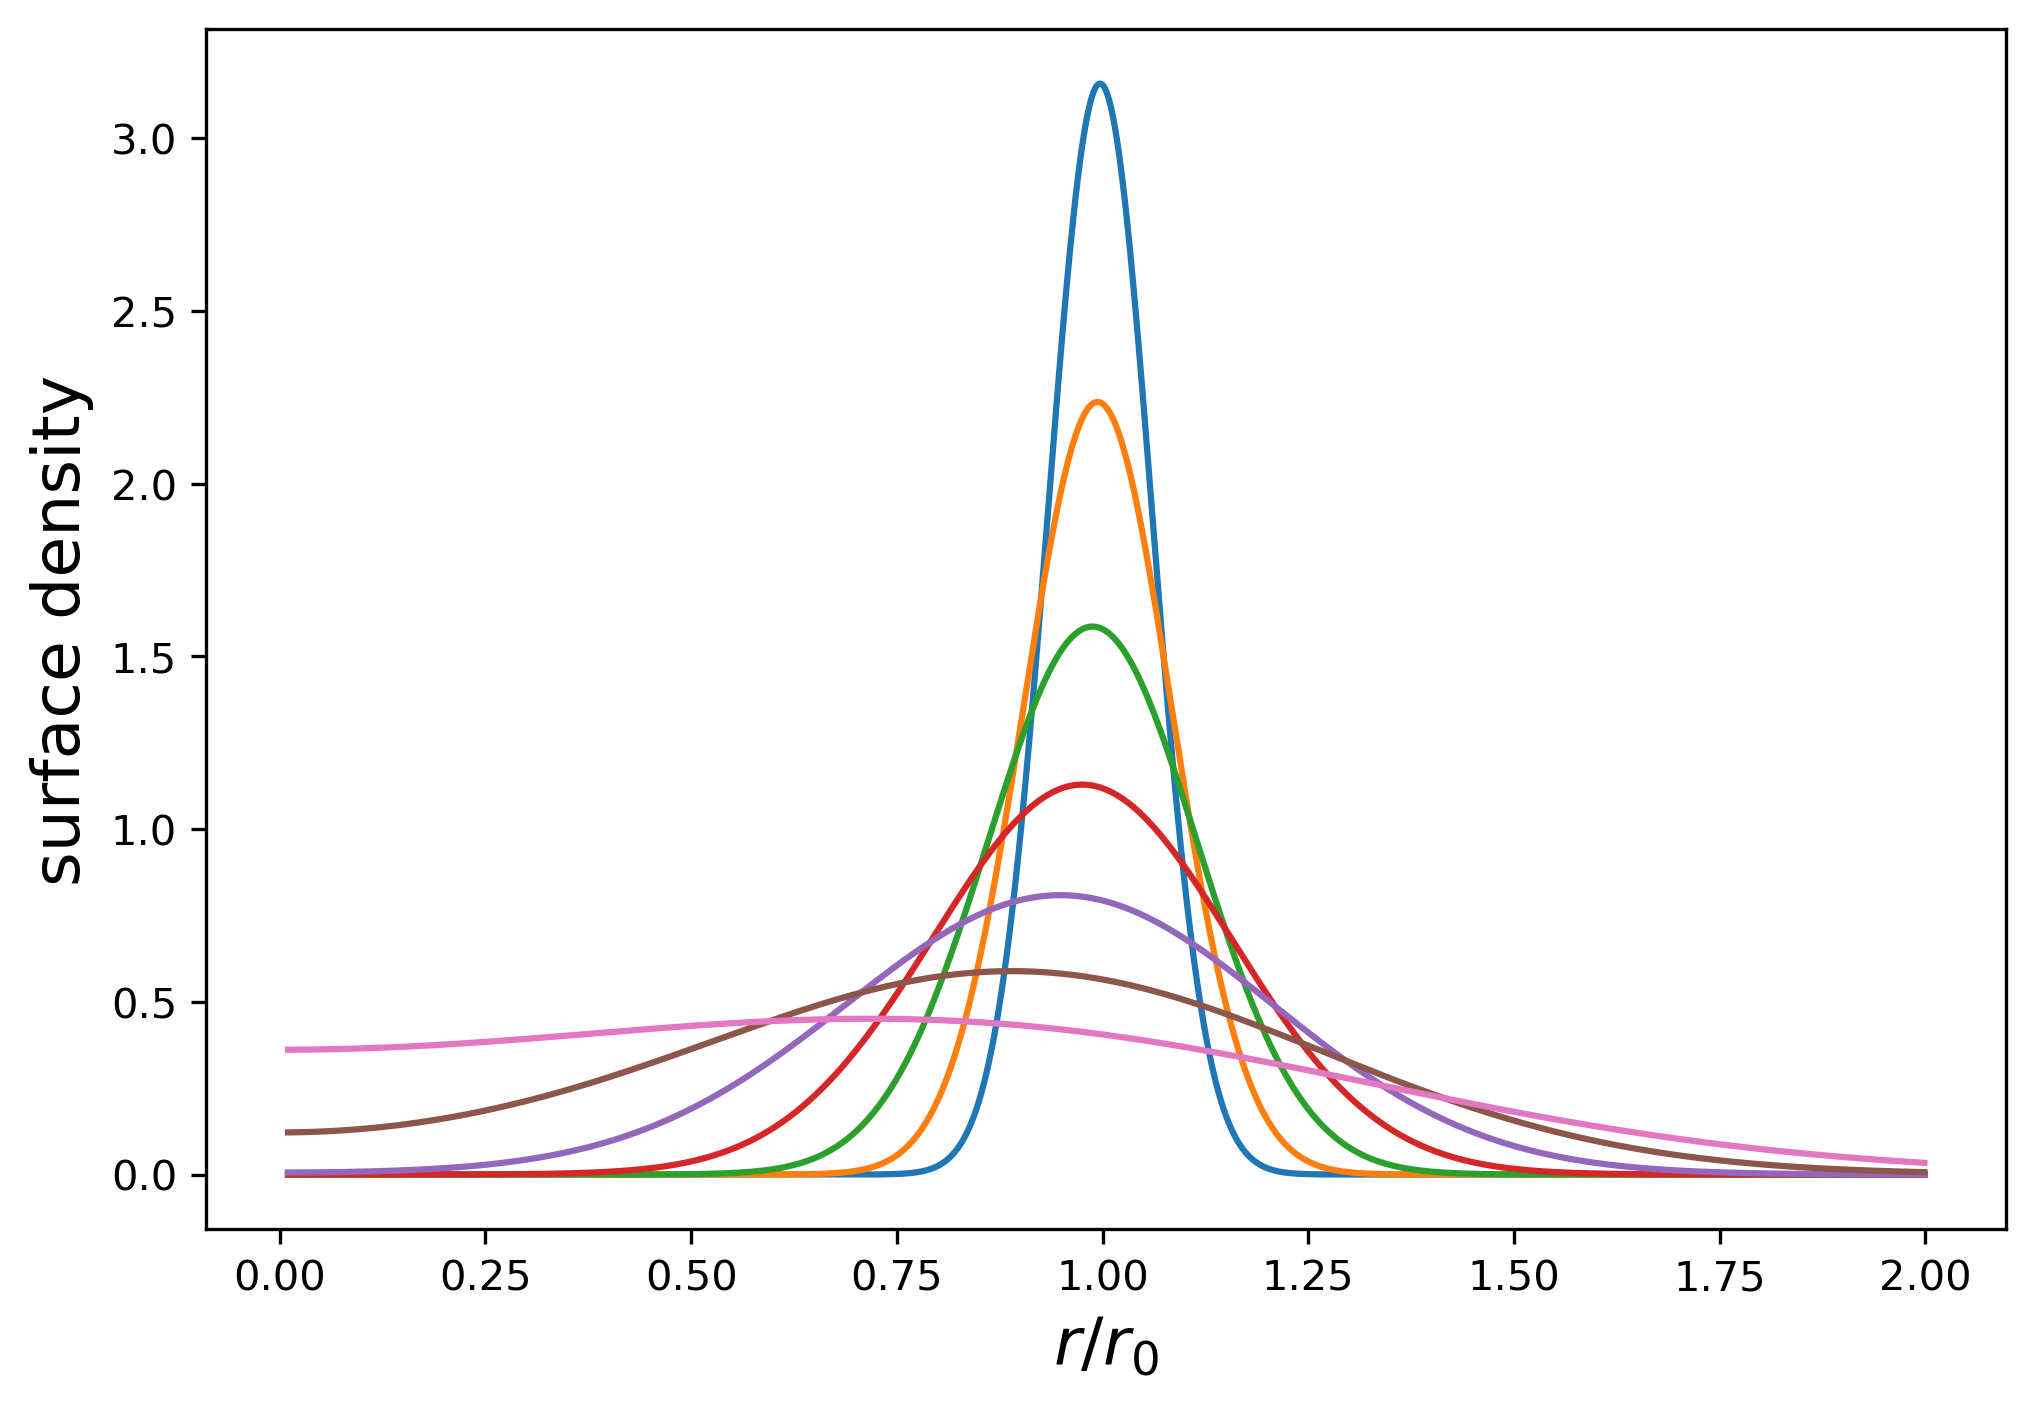
\includegraphics[width = 0.8\textwidth]{figures/armitage_ringspread.png}
    \caption{The evolution of a ring of gas centred initially at $r=r_0$ according to equation \ref{eq:1d_evol}, as derived by \citet{lynden-bell1974}. Each curve is plotted from $\tau=0.008$ to $\tau=0.512$ with interval 0.084, where $\tau$ is dimensionless time \citep[figure from lecture notes by][]{armitage2022}. The diffusive nature of the evolution is clearly evident, with the overdense ring spreading out over time.}
    \label{fig:ring_spreading}
\end{figure}

The analysis here and in section \ref{sec:fluid_eqns} relies on viscous disk theory as previously stated.
In this, we consider that although angular momentum may be physically transferred by mechanisms such as the magnerotational instability \citep{sano2000}, self-gravity \citep{kratter2016}, turbulent eddies \citep{klahr2003}, or others, we assume that all of the physics can be captured by the kinematic viscosity $\nu$.
Modelling disk evolution accurately therefore relies on determining the value of $\nu$.
\citet{shakura1973} argued that it is physically consistent to parametrise the viscosity in terms of some constant $\alpha \lesssim 1$ as\footnote{Strictly there is also a factor of $2/3$ on the right-hand side but this is typically ignored in the literature and absorbed into the value of $\alpha$.}
\begin{align}
    \nu = \alpha c H.
\end{align}
This is known as the $\alpha$\textit{-prescription}. If $\nu \propto r^\beta$ for some constant real number $\beta$, then \ref{eq:1d_evol} has solution \citep{lynden-bell1974}
\begin{align}
    \Sigma(r) = (2 - \beta) \frac{M_d}{2 \pi r_c^2} \left( \frac{r}{r_c} \right)^{-\beta} \exp{\left[ - \left(\frac{r}{r_c}\right)^{2-\beta} \right]}, \label{eq:exp_taper_dens}
\end{align}
which is a so-called \textit{exponentially tapered} power law in $\Sigma$.
That is, the density roughly obeys a negative power law with index $-\beta$ at radii less than the critical radius $r_c$, while dropping off exponentially at radii greater than $r_c$.
Using the $\alpha$-prescription and the definition of $\gamma$ given in equation \ref{eq:flared_hr} gives $\beta=2\gamma+\frac{1}{2}$.
More commonly this is parameterised in terms of the effective temperature profile or the sound speed profile $T \propto c^2 \propto r^{-2q}$ for some constant real number $q$, yielding $\beta = \frac{3}{2} - 2q$ \citep{hartmann1998}.
If we take $q=1/4$ as in section \ref{sec:disk_flaring}, then $\beta=1$ \citep{chiang1997}.

The exponentially tapered power law picture for the surface density profile \ref{eq:exp_taper_dens}, combined with the vertically Gaussian density structure \ref{eq:vertical_rho}, provide the typical parameterisation used to fit the density structure of observed disks \citep{andrews2011,zhang2021}.
The high-resolution MAPS survey found remarkably consistent best fitting parameters of $\beta=1$ and $\gamma=0.2$, with variation of only $\simeq20$\% and $\simeq10$\% respectively across the 5 disks in the sample.

\section{Observed Properties}

\subsection{Components}

Figure \ref{fig:struct_cartoon} presents a cartoon overview of the modern understanding of the structural components of protoplanetary disks \citep{andrews2020}.
The disk is comprised of both gas and dust, where dust is taken to mean any solid material.
The gas component is pressure supported and so exhibits the expected flared structure discussed in section \ref{sec:disk_flaring}.
The dust grains however do not feel any pressure and their behaviour depends on their size.
Small dust grains, those on the order of a few microns or less, couple strongly to the gas and thus trace the gas structure.
Larger grains experience drag forces and thus settle to the disk mid-plane \citep{nakagawa1986}.
These different components are probed via different observational tracers.
The distribution of small dust grains may be examined through scattered light, while the larger grains can be traced with millimetre thermal continuum observations \citep{almapartnership2015,andrews2016,ansdell2016}. 
The gas component on the other hand may be studied through spectral emission lines of different molecules.
These kinds of observations can be used to constrain the gas gas distribution \citep{vandermarel2015,ansdell2016,zhang2021}, kinematics \citep{perez2015,pinte2018a,teague2018,pinte2019,yu2021,calcino2022} and temperature \citep{pinte2018,calahan2021}.

\begin{figure}
    \centering
    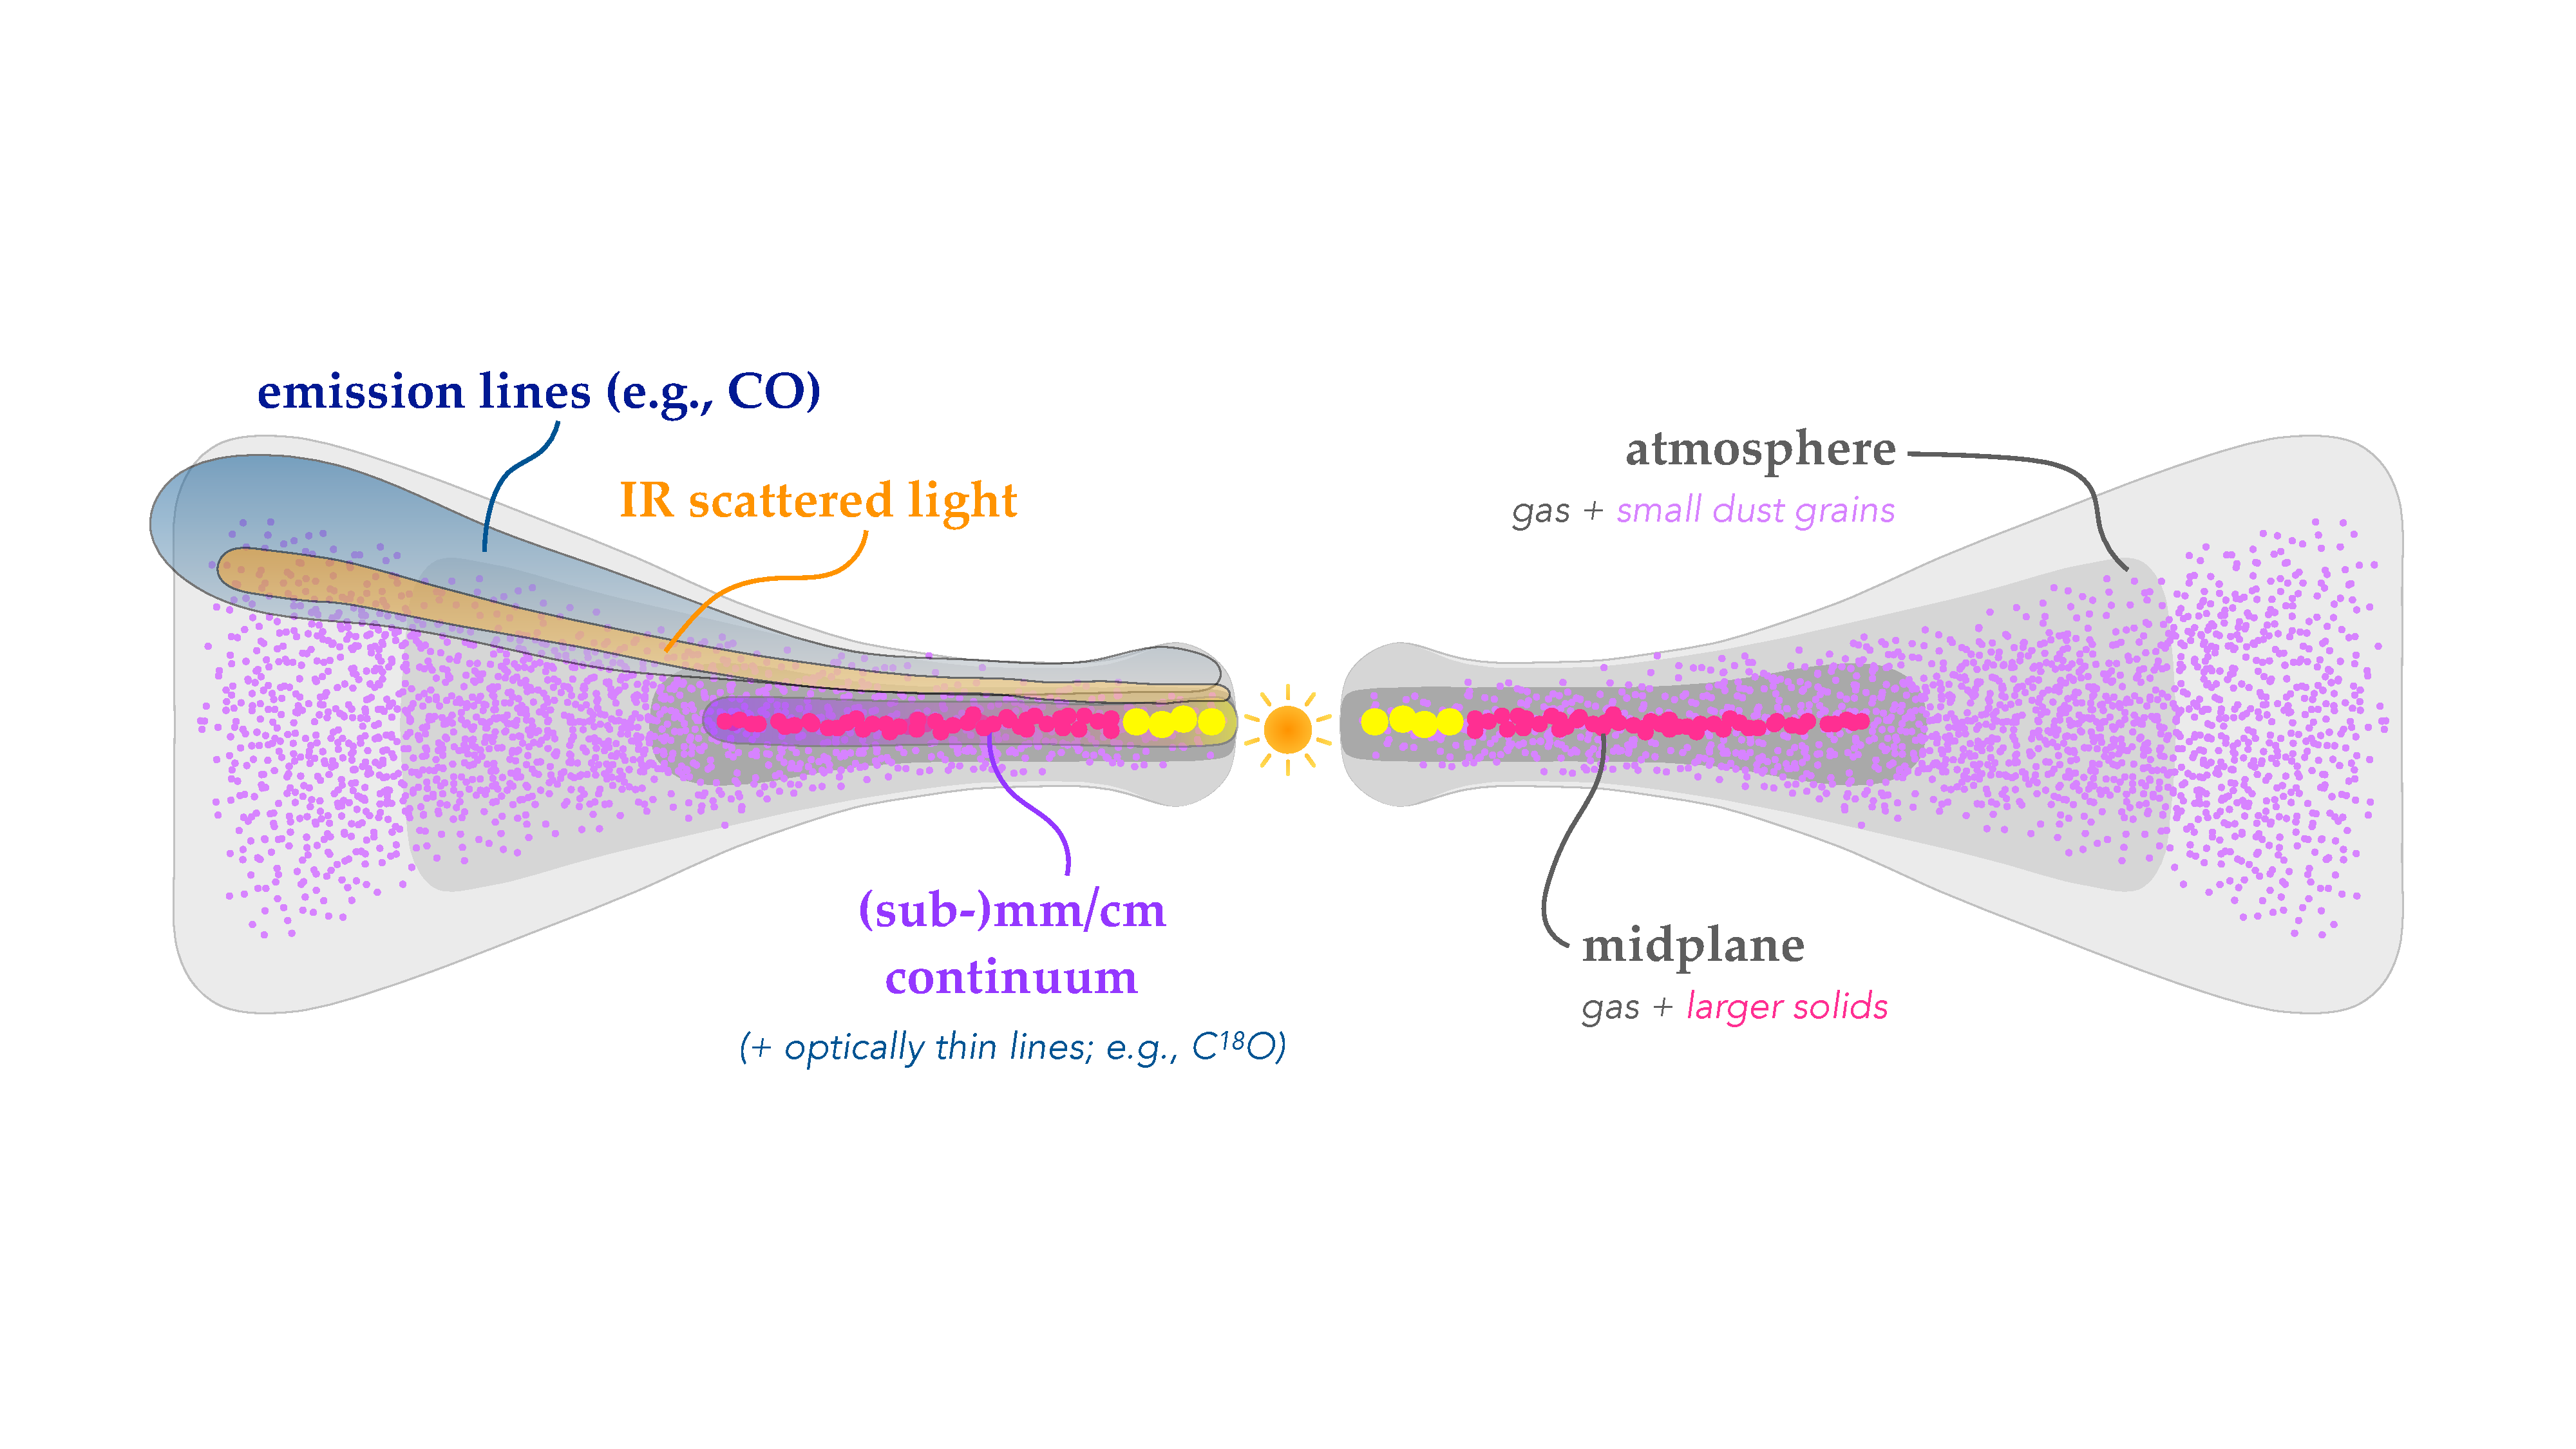
\includegraphics[width = 0.99\textwidth]{figures/cartoon_overview.pdf}
    \caption{A cross section schematic of a typical protoplanetary disk. The location of gas is shown in grey while dust grains and larger solids are shown in purple. Labels on the left outline key observational tracers of disk structure while the labels on the right identify those features. The figure is intended as a rough outline and is not to scale \citep[see review by][]{andrews2020}. The pressure support of the gas results in a thick disk extended in the vertical direction, while the large dust grains settle to a thin layer in the mid-plane.}
    \label{fig:struct_cartoon}
\end{figure}

\subsection{Size}

The size of a disk is typically defined as the radius within which 90\% of the total luminosity is contained.
This is in general a function of the observational tracer and so for example $R_\mathrm{mm}$ may be different to $R_\mathrm{CO}$, where the subscripts signify millimetre continuum and molecular carbon monoxide (CO) line emission respectively. 
Furthermore, each of these sizes may be used as a proxy for the size of a certain component of the disk based on what the component of the disk probes.
Thus $R_\mathrm{mm}$ is essentially the size of the dust disk comprised of millimetre sized grains and larger, while $R_\mathrm{CO}$ gives the size of the gas disk.
In general the size of the dust disk is smaller than the gas disk for the same system, as demonstrated in Figure \ref{fig:maps_disks}.
Medium resolution population studies that resolved almost 200 disks to scales of $25-50$ au suggest that the typical dust disk size is in the $\simeq 10 - 250$ au \citep{tripathi2017,andrews2018a,hendler2020}.
This range is supported by surveys of many fewer disks, around 30, taken at the much higher resolution of $\sim5$ au \citep{long2018,huang2018b}.
The gas disks are typically larger with radii of $100 - 500$ au, with a few extending out even farther \citep{ansdell2018,zhang2021}.

\begin{figure}
    \centering
    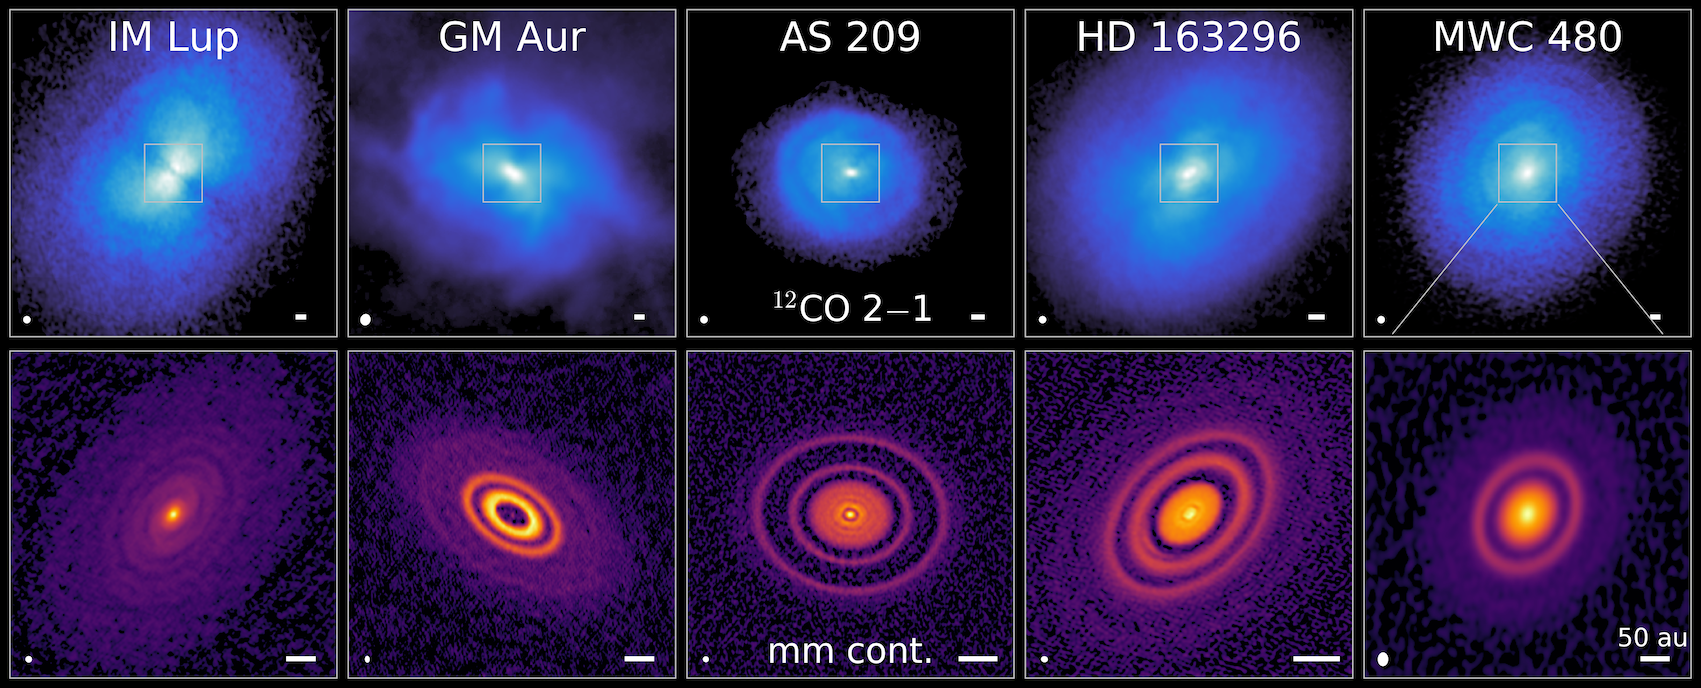
\includegraphics[width = 0.95\textwidth]{figures/Figure-DISKS-Website.png}
    \caption{Top row: $^{12}$CO $2-1$ Line emission integrated intensity images taken of the five protoplanetary disks as part of MAPS \citep{oberg2021}.
    The bottom row shows continuum millimetre observations of the same disks, zoomed in on the box shown on each figure in the top row \citep{andrews2018,huang2020,oberg2021}. 
    We see that in each case the spatial extent of the dust disk probed in mm is much less than that for the gas disk probed with $^{12}$CO.
    Figure retrieved from \url{https://www.alma-maps.info/disks.html}.}
    \label{fig:maps_disks}
\end{figure}

\subsection{Mass}

Observational disk mass measurements are something of a problem child.
We split the total disk mass $M_\mathrm{d}$ into two components, the gas mass $M_\mathrm{g}$  and the dust or solids mass $M_\mathrm{s}$ where $M_\mathrm{d} = M_\mathrm{g} + M_\mathrm{s}$.
Measurements of $M_\mathrm{s}$ rely on assumptions of the optical properties of dust grains and so are intrinsically uncertain.
$M_\mathrm{g}$ measurements are even worse off.
Molecular hydrogen is too faint in disks to be of use, no instruments operating or planned can observe the hydrogen deuteride $1-0$ transition that may be of use, and most other molecules are not very abundant.
CO is the next most abundant molecule after $H_2$ and is readily detectable at wavelengths available to ALMA.
Measurements of $M_\mathrm{g}$ via CO are unfortunately complicated by uncertainty in the C/H ratio in disks \citep[see the review by][for in-depth discussion of difficulties with disk mass measurements]{miotello2022}.

These measurements are crucial to understanding planet formation as they constrain the possible bodies that may be created from a disk as it continues to evolve.
The \textit{Minimum Mass Solar Nebula} (MMSN) is the hypothesised disk that the solar system formed from, with just enough mass to create each of the planets \citep{weidenschilling1977b,hayashi1981}.
Modern measurements place the MMSN at $M_\mathrm{s} \gtrsim 40 \, \mathrm{M_\oplus}$ (where $\mathrm{M_\oplus}$ is an Earth mass), $M_\mathrm{g} \gtrsim 3000 \, \mathrm{M_\oplus}$, where $\mathrm{M_\oplus}$ is an Earth mass \citep[see review by][]{andrews2020}.
If planets are formed from protoplanetary disks then the mass of said disks should be comparable to, or larger than, the MMSN.
Figure \ref{fig:disk_masses} shows the distribution of dust mass measurements for disks in the regions of Ophiuchus, Lupus, Upper Scorpius, Chamaeleon I, $\sigma$ Ori, IC 348 and Taurus \citep[and references therin]{cieza2019}, compared with the MMSN.
Even in the youngest regions of the sample, fewer than $20\%$ of the disks contain a dust mass greater than the MMSN value of $M_\mathrm{s}\gtrsim 40 \, \mathrm{M_\oplus}$.
This result does not seem to be compatible with the known population of exoplanets, a conundrum known as the \textit{missing mass problem} \citep[e.g.]{najita2014}.

One possible resolution to the missing mass problem is that protoplanetary disks are planet-hosting disks rather than planet-forming disks.
In this scenario planet formation occurs during the protostellar stage while the star is still embedded in a envelope, since massive disks are more common \citep{greaves2010}.
This scenario is supported by the growing body of evidence that protoplanetary disks contain planets when the system is as young as 1-2 Myr \citep{almapartnership2015,zhang2018,verrios2022}.
On the other hand planet formation may be incredibly efficient during the very early protoplanetary stage \citep{najita2014,manara2018,Tychoniec2020}.
A final possibility is that derived dust disk masses suffer from systematic underestimation. 
\citet{zhu2019} argued that if disks are not optically thin, as assumed in calculations of disk mass from continuum observations, then the true dust mass may be a factor of 2 or more larger.
Whatever the case may be, it is likely that detecting young planets and constraining their masses through kinematic observations will be a key part of determining which scenario is correct.

\begin{figure}
    \centering
    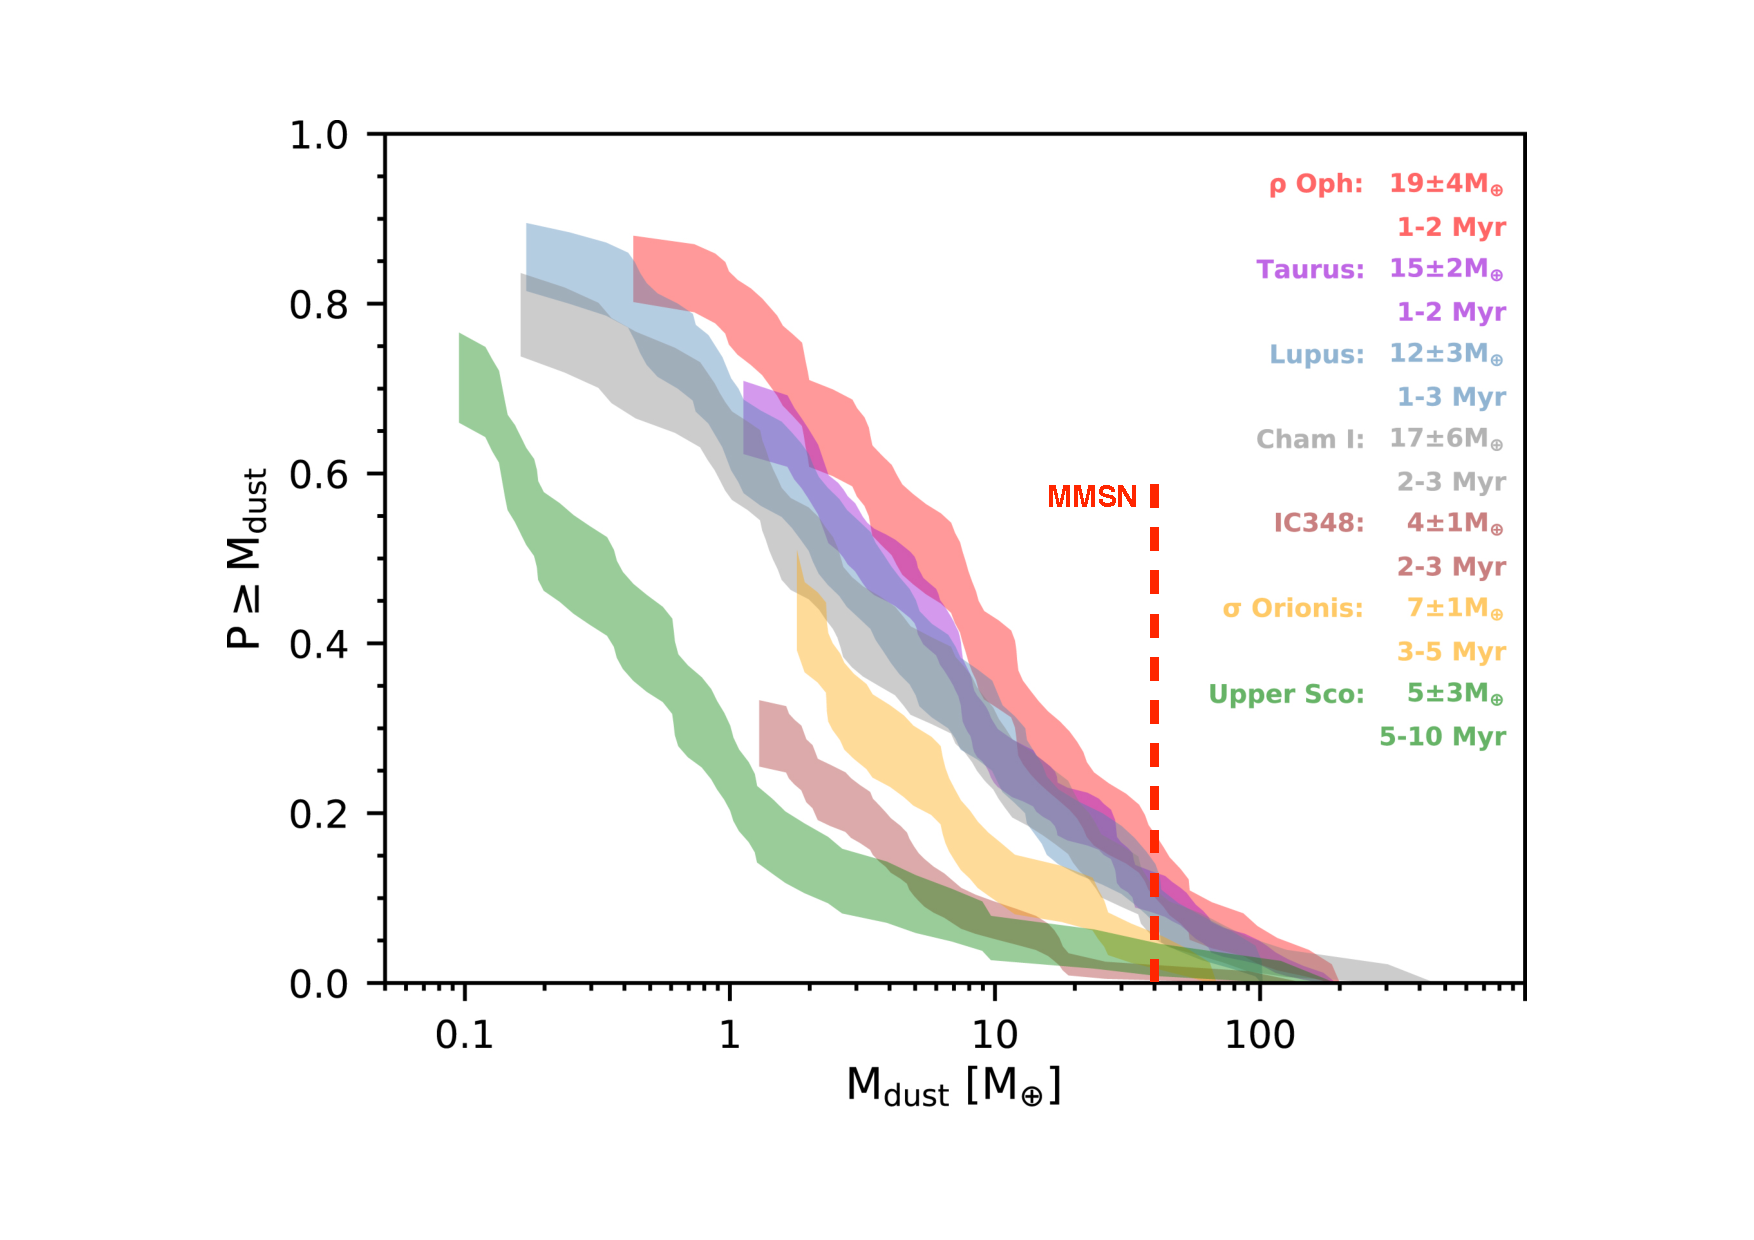
\includegraphics[width = 0.7\textwidth]{figures/disk_mass.pdf}
    \caption{Cumulative mass distributions for disks found in various nearby young stellar regions. The shaded regions represent the $1\sigma$ confidence intervals \citep{vanterwisga2019}. Plotted in red is the dust mass of the MMSN \citep{weidenschilling1977b}. According to this analysis, very few of the disks in the sample have enough mass to create the planets of the solar system.}
    \label{fig:disk_masses}
\end{figure}